% Taller 1 - Teoria de Aprendizaje de Maquina 2026-2
% Documento de solucion. Compilar con: pdflatex informe.tex (dos veces)
\documentclass[11pt,a4paper]{article}

\usepackage[utf8]{inputenc}
\usepackage[T1]{fontenc}
\usepackage[spanish,es-noshorthands]{babel}
\usepackage{lmodern}
\usepackage{microtype}
\usepackage[margin=2.4cm]{geometry}
\usepackage{amsmath,amssymb,amsthm}
\usepackage{graphicx}
\usepackage{booktabs}
\usepackage{array}
\usepackage{float}
\usepackage{caption}
\usepackage{subcaption}
\usepackage{enumitem}
\usepackage{xcolor}
\usepackage{listings}
\usepackage[hidelinks]{hyperref}

\graphicspath{{../figuras/}}

\definecolor{codebg}{gray}{0.96}
\definecolor{codekw}{RGB}{0,90,160}
\definecolor{codecm}{RGB}{90,120,90}
\lstset{
  language=Python,
  basicstyle=\ttfamily\footnotesize,
  backgroundcolor=\color{codebg},
  keywordstyle=\color{codekw}\bfseries,
  commentstyle=\color{codecm}\itshape,
  stringstyle=\color{orange!70!black},
  numbers=left, numberstyle=\tiny\color{gray}, numbersep=6pt,
  frame=single, rulecolor=\color{gray!50},
  breaklines=true, showstringspaces=false,
  columns=fullflexible, keepspaces=true,
  xleftmargin=1.4em, framexleftmargin=1.2em,
  literate={á}{{\'a}}1 {é}{{\'e}}1 {í}{{\'i}}1 {ó}{{\'o}}1 {ú}{{\'u}}1
           {ñ}{{\~n}}1 {Á}{{\'A}}1 {Í}{{\'I}}1 {Ó}{{\'O}}1 {Ú}{{\'U}}1 {Ñ}{{\~N}}1
}

\captionsetup{font=small,labelfont=bf}
\setlist{itemsep=2pt,topsep=3pt}
\newcommand{\R}{\mathbb{R}}
\newcommand{\x}{\mathbf{x}}
\newcommand{\w}{\mathbf{w}}
\newcommand{\yhat}{\hat y}

\title{\textbf{Taller 1: Teoría de Aprendizaje de Máquina -- 2026-2}\\[4pt]
\large Clasificación supervisada, vecinos cercanos y evaluación de modelos}
\author{Cristian David Dorado Gómez\\[2pt]
\small Profesor: Diego Armando Pérez Rosero}
\date{\today}

\begin{document}
\maketitle

\begin{abstract}
\noindent
Se resuelven los tres puntos del taller: (1) clasificación lineal con el
perceptrón, incluyendo la frontera de decisión, la demostración de crecimiento
del margen y un ejercicio numérico; (2) clasificación por $k$ vecinos más
cercanos, con el cálculo manual de distancias y votación, y la evaluación
experimental sobre \texttt{make\_moons} ($N=300$, \texttt{noise=0.20},
\texttt{random\_state=42}); y (3) evaluación de un clasificador binario con
matriz de confusión, métricas manuales y verificación en \texttt{scikit-learn}.
Todos los resultados numéricos de este documento provienen de la ejecución del
cuaderno reproducible \texttt{solucion\_taller.ipynb}, con semillas fijas
(\texttt{np.random.seed(42)}).
\end{abstract}

\tableofcontents
\vspace{0.5cm}

%==========================================================================
\section{Punto 1: clasificación lineal y algoritmo del perceptrón}

El clasificador binario asigna
\begin{equation}
\yhat =
\begin{cases}
+1, & \w^\top \x + b > 0,\\
-1, & \w^\top \x + b \le 0,
\end{cases}
\qquad \w \in \R^2,\; b \in \R ,
\end{equation}
es decir, $\yhat = \operatorname{sign}(\w^\top \x + b)$ con la convención de que el
valor $0$ se asigna a la clase $-1$. La función $f(\x) = \w^\top \x + b$ es el
\emph{puntaje} o función de decisión: su signo da la clase y su magnitud
(absoluta, dividida por $\lVert \w \rVert$) la distancia a la frontera.

\subsection{Frontera de decisión}

Con $\w = (1,2)^\top$ y $b = -3$ la frontera $\w^\top \x + b = 0$ es
\begin{equation}
x_1 + 2x_2 - 3 = 0
\quad\Longleftrightarrow\quad
x_2 = \frac{3 - x_1}{2} = 1.5 - 0.5\,x_1 ,
\end{equation}
una recta de pendiente $-1/2$ que corta el eje $x_1$ en $x_1 = 3$ y el eje $x_2$
en $x_2 = 1.5$. El vector $\w = (1,2)^\top$ es \emph{normal} a la recta y apunta
hacia el semipiano de la clase $+1$: la región $x_1 + 2x_2 > 3$ es la clase $+1$
y $x_1 + 2x_2 < 3$ es la clase $-1$; la recta misma pertenece a $-1$ por la
convención $\le 0$. La Figura~\ref{fig:frontera} muestra la recta y los cuatro
puntos.

\begin{figure}[H]
  \centering
  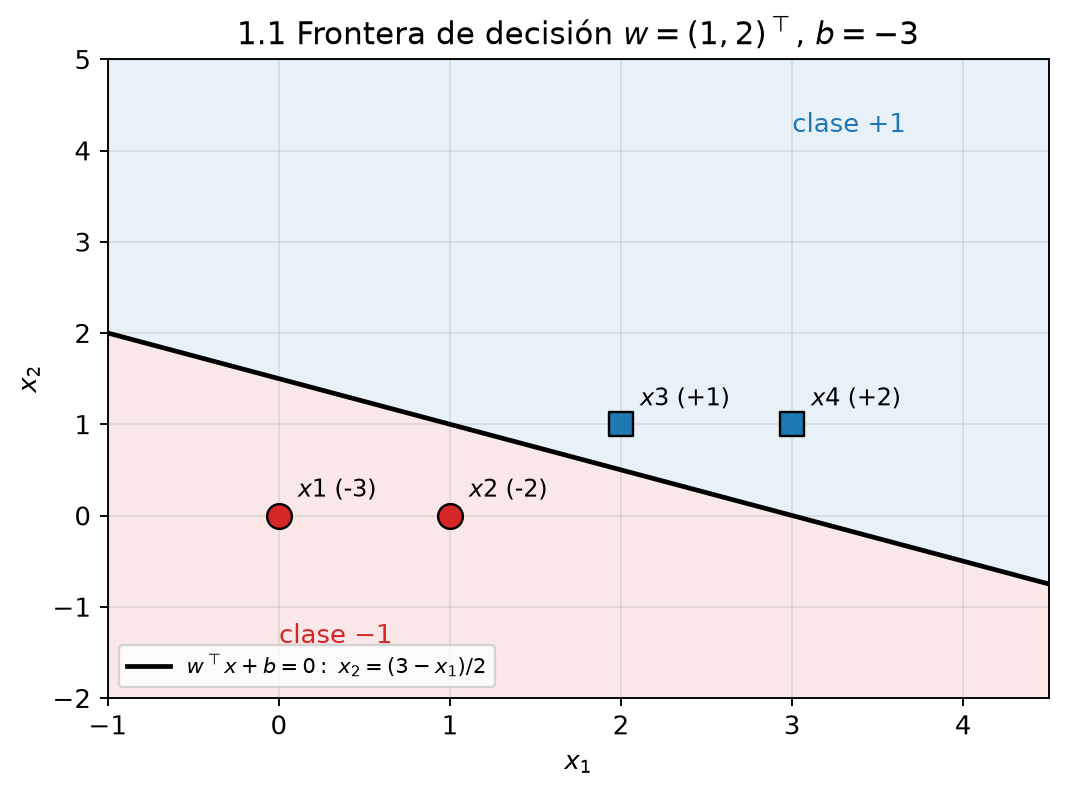
\includegraphics[width=0.68\textwidth]{fig_1_1_frontera.png}
  \caption{1.1 Frontera de decisión para $\w=(1,2)^\top$, $b=-3$ y clasificación de
  $x_1,\dots,x_4$. El valor entre paréntesis es $f(\x)=\w^\top\x+b$.}
  \label{fig:frontera}
\end{figure}

Sustituyendo cada punto en $f(\x) = x_1 + 2x_2 - 3$ se obtiene la
Tabla~\ref{tab:punto11}. La justificación de cada predicción es simplemente el
signo de $f$: no se requiere otra regla.

\begin{table}[H]
\centering
\caption{1.1 Evaluación de la regla de decisión en los cuatro puntos.}
\label{tab:punto11}
\begin{tabular}{lcccc}
\toprule
Observación & $\x$ & $f(\x) = x_1 + 2x_2 - 3$ & Signo & $\yhat$ \\
\midrule
$x_1$ & $(0,0)$ & $0+0-3 = -3$ & $<0$ & $-1$ \\
$x_2$ & $(1,0)$ & $1+0-3 = -2$ & $<0$ & $-1$ \\
$x_3$ & $(2,1)$ & $2+2-3 = +1$ & $>0$ & $+1$ \\
$x_4$ & $(3,1)$ & $3+2-3 = +2$ & $>0$ & $+1$ \\
\bottomrule
\end{tabular}
\end{table}

\noindent
Las distancias a la frontera son $\lvert f(\x)\rvert/\lVert \w \rVert$ con
$\lVert \w \rVert = \sqrt{5} \approx 2.2361$: $1.3416$ y $0.8944$ para $x_1$ y
$x_2$ (lado negativo), y $0.4472$ y $0.8944$ para $x_3$ y $x_4$ (lado positivo).
Los dos puntos negativos están más lejos de la frontera que $x_3$, que es el
punto positivo más cercano a ella.

\subsection{Actualización del perceptrón y el margen}

Con la regla
\begin{equation}
\w_{\text{nuevo}} = \w + \eta\,y_i\,\x_i, \qquad
b_{\text{nuevo}} = b + \eta\,y_i, \qquad \eta > 0,
\end{equation}
y el margen $m_i = y_i\,(\w^\top \x_i + b)$, el margen de la misma observación
inmediatamente después de la actualización es
\begin{align}
m_{i,\text{nuevo}}
&= y_i\left(\w_{\text{nuevo}}^\top \x_i + b_{\text{nuevo}}\right) \nonumber\\
&= y_i\left((\w + \eta\,y_i\,\x_i)^\top \x_i + b + \eta\,y_i\right) \nonumber\\
&= y_i\left(\w^\top \x_i + b\right)
 + \eta\,y_i\,\big(y_i\,\x_i^\top \x_i\big)
 + \eta\,y_i^2 \nonumber\\
&= m_i + \eta\,y_i^2\lVert \x_i\rVert_2^2 + \eta\,y_i^2 .
\end{align}
Como $y_i \in \{-1,+1\}$, se tiene $y_i^2 = 1$ y por lo tanto
\begin{equation}
\boxed{\;m_{i,\text{nuevo}} = m_i + \eta\left(\lVert \x_i\rVert_2^2 + 1\right)\;}
\qquad \text{con } \eta\left(\lVert \x_i\rVert_2^2 + 1\right) > 0 .
\end{equation}

\paragraph{Qué implica.} El incremento es \emph{estrictamente positivo} y
\emph{no depende del valor previo de $m_i$}: sin importar cuán mal clasificada
esté la observación, la actualización la desplaza siempre hacia el lado correcto
de la frontera en una cantidad fija (que crece con $\lVert \x_i\rVert^2$). Dicho
de otro modo, el error cometido sobre esa observación se corrige en la dirección
correcta y el perceptrón «refuerza» la etiqueta verdadera $y_i$.

Dos precisiones que conviene explicitar:
\begin{itemize}
\item El margen \emph{geométrico} es $m_i/\lVert \w \rVert$. El numerador crece,
  pero $\lVert \w \rVert$ también cambia con cada actualización, de modo que el
  margen geométrico no es necesariamente monótono; la fórmula garantiza el
  crecimiento del margen funcional.
\item Una sola actualización no basta para que un punto muy mal clasificado quede
  bien clasificado: el desplazamiento es fijo, mientras que $-\eta m_i$ puede ser
  mucho mayor. Lo que garantiza la fórmula es el avance constante, y es la base
  de la cota de convergencia del perceptrón: si los datos son linealmente
  separables con margen geométrico $\gamma$ y $R=\max_i\lVert \x_i\rVert$, el
  número de errores está acotado por $(R/\gamma)^2$.
\end{itemize}

Verificación numérica (celda de código del cuaderno, cinco casos aleatorios con
error forzado): en todos se cumple
$\lvert m_{i,\text{nuevo}} - (m_i + \eta(\lVert\x_i\rVert^2+1))\rvert < 10^{-12}$
y $m_{i,\text{nuevo}} > m_i$; por ejemplo, para un caso con
$m_i = -1.5102$ y $\eta = 0.5$ el margen nuevo es $1.7409$, exactamente
$m_i + \eta(\lVert \x_i\rVert^2+1)$.

\subsection{Ejercicio numérico}

Datos: $\w = (0,0)^\top$, $b = 0$, $\eta = 0.5$, $\x = (2,1)^\top$, $y = +1$.

\paragraph{Paso 1: ¿hay error?} El puntaje es
$f(\x) = 0\cdot 2 + 0\cdot 1 + 0 = 0$. La regla de predicción asigna $+1$ sólo si
$f(\x) > 0$; como $0$ no es mayor que cero, $\yhat = -1$. Con $y = +1$ y
$\yhat = -1$ la observación está mal clasificada (margen
$m = y\,f(\x) = 0 \le 0$); \textbf{sí corresponde actualizar}.

\paragraph{Paso 2: actualización} con $\eta\,y = 0.5\cdot(+1) = 0.5$:
\begin{equation}
\w_{\text{nuevo}} =
\begin{pmatrix} 0\\0\end{pmatrix}
+ 0.5\,(+1)\begin{pmatrix} 2\\1\end{pmatrix}
= \begin{pmatrix} 1\\0.5\end{pmatrix},
\qquad
b_{\text{nuevo}} = 0 + 0.5\,(+1) = 0.5 .
\end{equation}

\paragraph{Paso 3: nuevo margen}
\begin{equation}
m_{\text{nuevo}} = y\left(\w_{\text{nuevo}}^\top \x + b_{\text{nuevo}}\right)
= (+1)\left(1\cdot 2 + 0.5\cdot 1 + 0.5\right) = 3 .
\end{equation}
Comprobación con la fórmula de 1.2:
$m + \eta(\lVert \x\rVert_2^2 + 1) = 0 + 0.5\,(4+1+1) = 3$. \checkmark\\
El nuevo puntaje es $+3 > 0$, así que la observación queda bien clasificada, con
margen funcional $3$ y margen geométrico
$3/\lVert \w_{\text{nuevo}}\rVert = 3/\sqrt{1.25} \approx 2.6833$.

%==========================================================================
\section{Punto 2: clasificación por los $k$ vecinos más cercanos}

Observación nueva $q = (1,1)$ y conjunto de entrenamiento

\begin{table}[H]
\centering
\begin{tabular}{lccccc}
\toprule
Observación & $x_1$ & $x_2$ & $x_3$ & $x_4$ & $x_5$\\
\midrule
$\x_i$ & $(0,0)$ & $(1,0)$ & $(3,1)$ & $(0,3)$ & $(1.1,\,1.1)$\\
Clase    & A & A & B & B & B\\
\bottomrule
\end{tabular}
\end{table}

\subsection{Cálculo manual de distancias y votación}

Con la distancia euclidiana
$d(q,\x_i) = \sqrt{(q_1 - x_{i,1})^2 + (q_2 - x_{i,2})^2}$:
\begin{align*}
d(q,\x_1) &= \sqrt{(1-0)^2 + (1-0)^2} = \sqrt{2} \approx 1.4142,\\
d(q,\x_2) &= \sqrt{(1-1)^2 + (1-0)^2} = \sqrt{1} = 1.0000,\\
d(q,\x_3) &= \sqrt{(1-3)^2 + (1-1)^2} = \sqrt{4} = 2.0000,\\
d(q,\x_4) &= \sqrt{(1-0)^2 + (1-3)^2} = \sqrt{5} \approx 2.2361,\\
d(q,\x_5) &= \sqrt{(1-1.1)^2 + (1-1.1)^2} = \sqrt{0.02} \approx 0.1414 .
\end{align*}

Todas las distancias son distintas, de modo que el orden es único y no hay
empates que romper (Tabla~\ref{tab:distancias}, Figura~\ref{fig:distancias}).

\begin{table}[H]
\centering
\caption{2.1 Orden de cercanía a $q=(1,1)$ y votación mayoritaria.}
\label{tab:distancias}
\begin{tabular}{clccl}
\toprule
Puesto & Observación & Distancia & Clase & \\
\midrule
1 & $x_5 = (1.1,1.1)$ & $0.1414$ & B & \\
2 & $x_2 = (1,0)$     & $1.0000$ & A & \\
3 & $x_1 = (0,0)$     & $1.4142$ & A & \\
4 & $x_3 = (3,1)$     & $2.0000$ & B & \\
5 & $x_4 = (0,3)$     & $2.2361$ & B & \\
\midrule
\multicolumn{5}{l}{$k=1$: $\{x_5\}$ $\rightarrow$ A: 0, B: 1 $\rightarrow$ $\yhat = $ \textbf{B}}\\
\multicolumn{5}{l}{$k=3$: $\{x_5,x_2,x_1\}$ $\rightarrow$ A: 2, B: 1 $\rightarrow$ $\yhat = $ \textbf{A}}\\
\multicolumn{5}{l}{$k=5$: todos $\rightarrow$ A: 2, B: 3 $\rightarrow$ $\yhat = $ \textbf{B}}\\
\bottomrule
\end{tabular}
\end{table}

\begin{figure}[H]
\centering
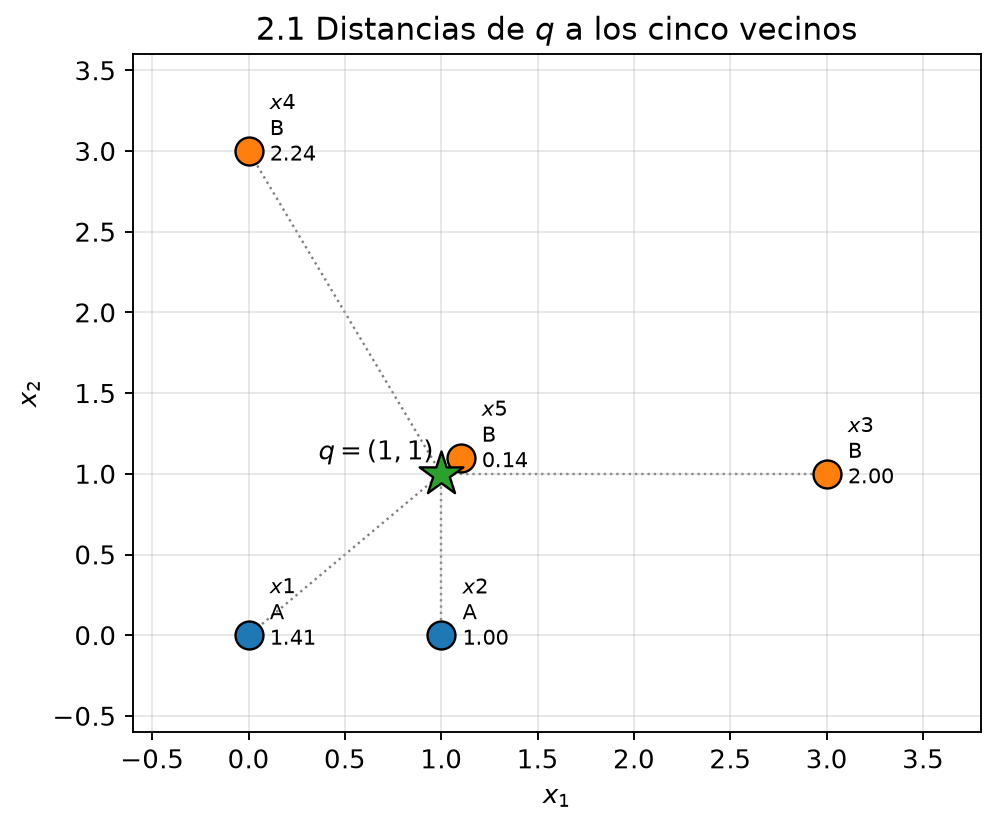
\includegraphics[width=0.55\textwidth]{fig_2_1_distancias.png}
\caption{2.1 Distancias de $q$ a los cinco vecinos (la etiqueta bajo cada punto
indica clase y distancia).}
\label{fig:distancias}
\end{figure}

\paragraph{Por qué $k$ puede cambiar la predicción.} El vecino más cercano, $x_5$,
está a $0.1414$ de $q$ y es de clase B: un punto casi pegado a $q$. Con $k=3$
entran $x_2$ y $x_1$, ambos A, que son mayoría y anulan el voto de $x_5$; con
$k=5$ se incorporan $x_3$ y $x_4$, ambos B, y la mayoría (3 a 2) depende ahora de
puntos a más de dos unidades de $q$, es decir, de la tendencia global del
conjunto y no de la vecindad local de $q$. En general, $k$ controla el compromiso
sesgo--varianza: $k$ pequeño usa sólo la vecindad inmediata (fronteras
irregulares, muy sensibles al ruido); $k$ grande promedia sobre una región amplia
(fronteras suaves, pero puede diluir la estructura local y arrastrar la clase
mayoritaria). Aquí, con $N=5$ y sin empates, la predicción «oscila» B $\to$ A
$\to$ B.

\subsection{Implementación sobre \texttt{make\_moons}}

\paragraph{Protocolo.} $N=300$ observaciones bidimensionales generadas con
\texttt{make\_moons(n\_samples=300, noise=0.20, random\_state=42)}; partición
70\,\% entrenamiento ($210$ observaciones) y 30\,\% prueba ($90$),
estratificada con \texttt{random\_state=42}, de modo que cada subconjunto conserva
50\,\%/50\,\% de clases; \texttt{KNeighborsClassifier} con
$k \in \{1,5,15\}$, distancia euclidiana y votación uniforme (valores por
defecto). Se reporta exactitud (\emph{accuracy}) en entrenamiento y en prueba
(Tabla~\ref{tab:acc}), y se dibujan los datos (Figura~\ref{fig:datos}) y las
regiones de decisión para $k=1$ y $k=15$ (Figura~\ref{fig:regiones}).

\begin{table}[H]
\centering
\caption{2.2 Exactitud de k-NN sobre \texttt{make\_moons} (210 entrenamiento /
90 prueba).}
\label{tab:acc}
\begin{tabular}{ccc}
\toprule
{$k$} & Exactitud entrenamiento & Exactitud prueba \\
\midrule
1  & 1.0000 & 0.9333 \\
5  & 0.9571 & \textbf{0.9556} \\
15 & 0.9571 & 0.9333 \\
\bottomrule
\end{tabular}
\end{table}

\begin{figure}[H]
\centering
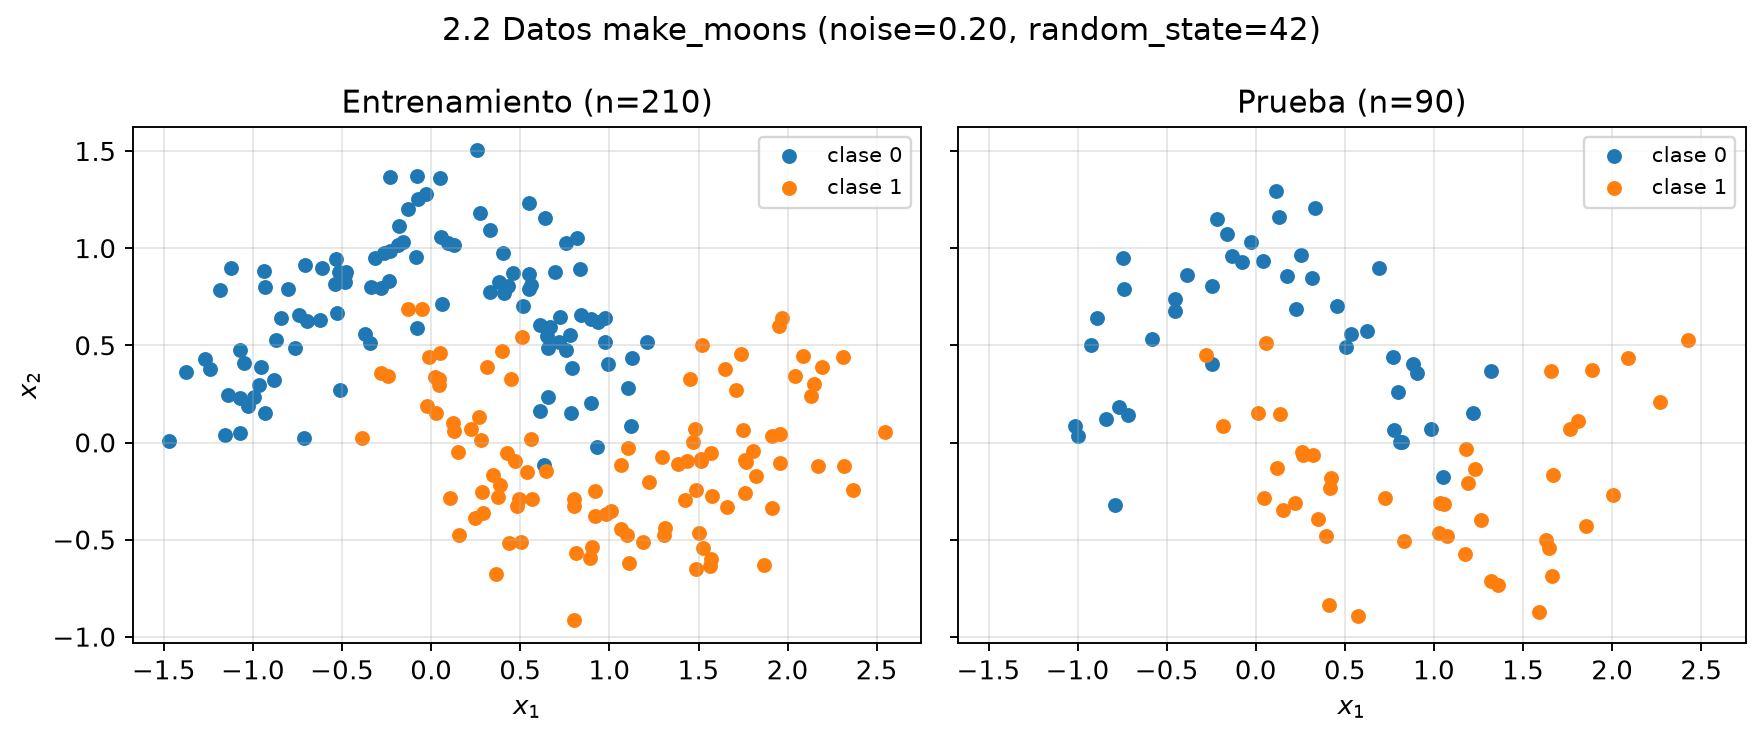
\includegraphics[width=\textwidth]{fig_2_2_datos.png}
\caption{2.2 Datos de \texttt{make\_moons} separados en entrenamiento y prueba.}
\label{fig:datos}
\end{figure}

\begin{figure}[H]
\centering
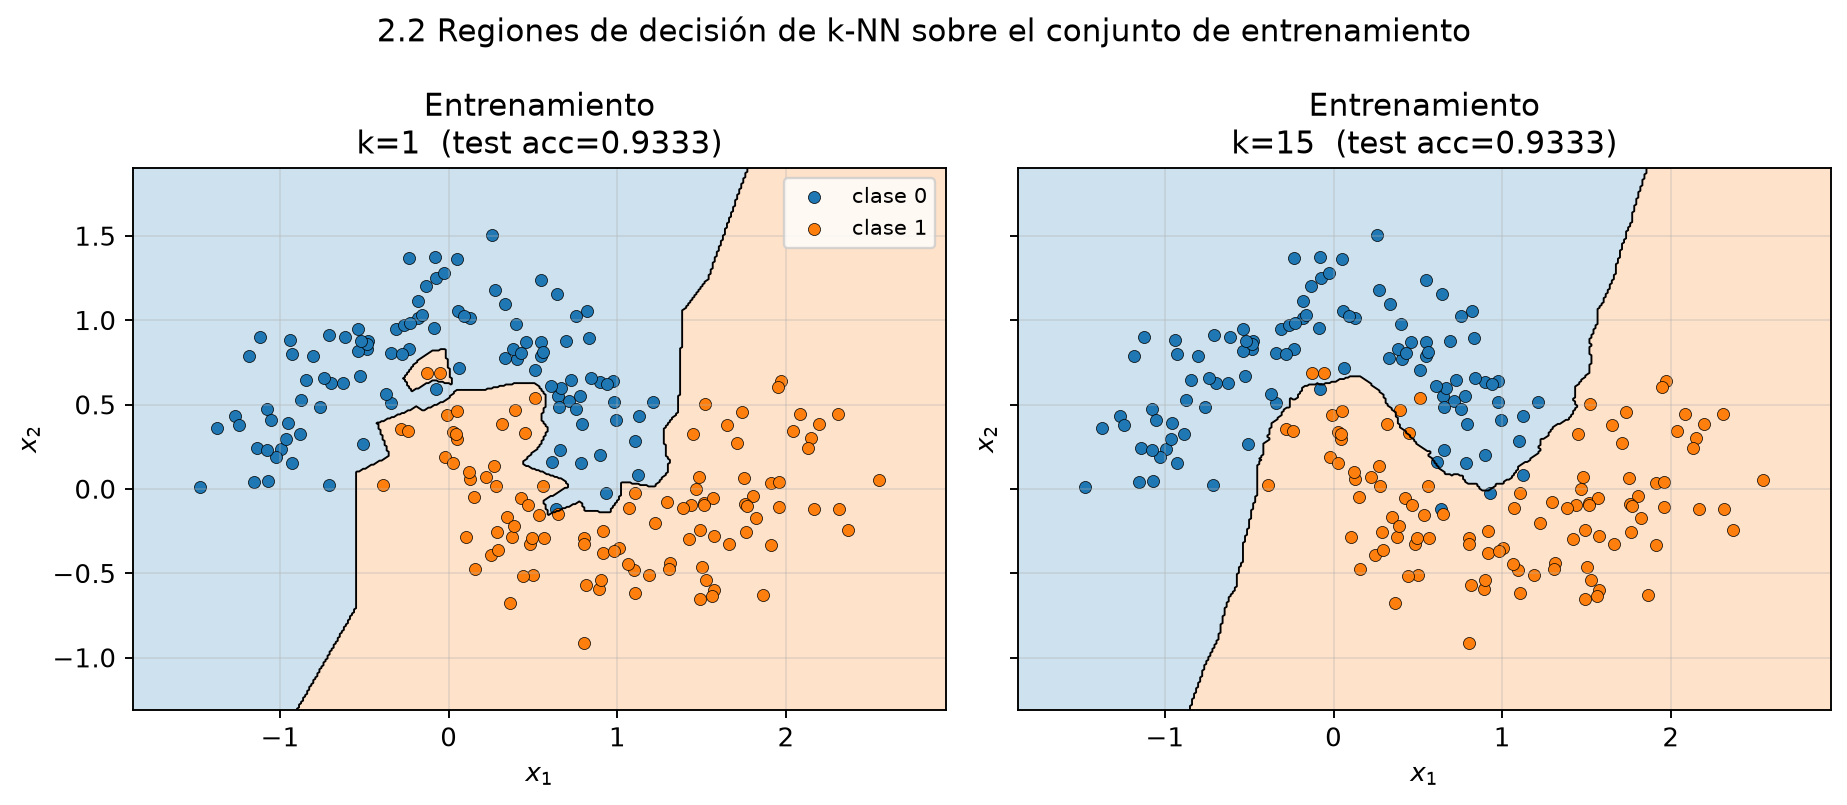
\includegraphics[width=\textwidth]{fig_2_2_regiones.png}
\caption{2.2 Regiones de decisión para $k=1$ (izquierda) y $k=15$ (derecha) sobre
el conjunto de entrenamiento. Con $k=1$ la frontera se ajusta a cada punto
(incluidos los ruidosos); con $k=15$ es más suave.}
\label{fig:regiones}
\end{figure}

\subsection{Interpretación}

\paragraph{$k$ muy pequeño.} Con $k=1$ cada observación se clasifica según su
vecino inmediato, así que la exactitud de entrenamiento es $1.0000$ por
construcción (cada punto es su propio vecino más cercano). Es un modelo de
\emph{varianza alta}: la frontera es muy irregular, se amolda al ruido
(Figura~\ref{fig:regiones}, izquierda) y pequeñas perturbaciones de los datos
cambian mucho la predicción; pueden aparecer islas de una clase dentro de la otra.

\paragraph{$k$ muy grande.} Al promediar muchos vecinos, la frontera se suaviza y
se vuelve estable, pero el sesgo aumenta: si $k$ es comparable con el tamaño de la
muestra, la vecindad cubre casi todo el espacio y la predicción tiende a la clase
mayoritaria, perdiendo la estructura de las dos lunas. Con $k=15$ ya se observa
una frontera notoriamente más limpia.

\paragraph{Cuál generalizó mejor.} Las exactitudes de prueba son $0.9333$ ($k=1$),
$0.9556$ ($k=5$) y $0.9333$ ($k=15$): el mejor de los tres es $k=5$
($86/90$ aciertos). La justificación no es la exactitud de entrenamiento —que
siempre favorece a $k=1$— sino el desempeño sobre datos no vistos: $k=1$ sufre el
ruido de los puntos de la frontera entre las lunas y $k=15$ suaviza tanto que
pierde puntos de las «colas»; $k=5$ conserva la estructura local y descarta el
ruido puntual. Las diferencias son pequeñas (una o dos observaciones de prueba),
lo que indica que con \texttt{noise=0.20} el problema es relativamente sencillo
para k-NN.

\paragraph{Por qué $k$ debe elegirse con validación y no con prueba.} La exactitud
de prueba estima el desempeño de un modelo \emph{ya elegido} sobre datos que el
procedimiento no utilizó. Si se prueban muchos valores de $k$ y se escoge el que
maximiza la exactitud de prueba, ese conjunto deja de ser una muestra
independiente: el número reportado queda sesgado de forma optimista y sobreestima
el desempeño real (fuga de información desde el conjunto de evaluación hacia la
selección del modelo). El procedimiento correcto es seleccionar $k$ \emph{dentro}
del conjunto de entrenamiento con validación cruzada estratificada (o con un
conjunto de validación aparte) y reservar el conjunto de prueba para un único
reporte final. La Figura~\ref{fig:cv} muestra esa selección con 5 pliegues sobre
las 210 observaciones de entrenamiento, para $k$ impar entre 1 y 39: el máximo de
la exactitud media de validación se alcanza en $k=11$ ($0.9619$), y su exactitud
de prueba, reportada una sola vez, es $0.9667$. Nótese que esta cifra no se usó
para elegir $k$: si se hubiera hecho así, el valor reportado habría sido
optimista.

\begin{figure}[H]
\centering
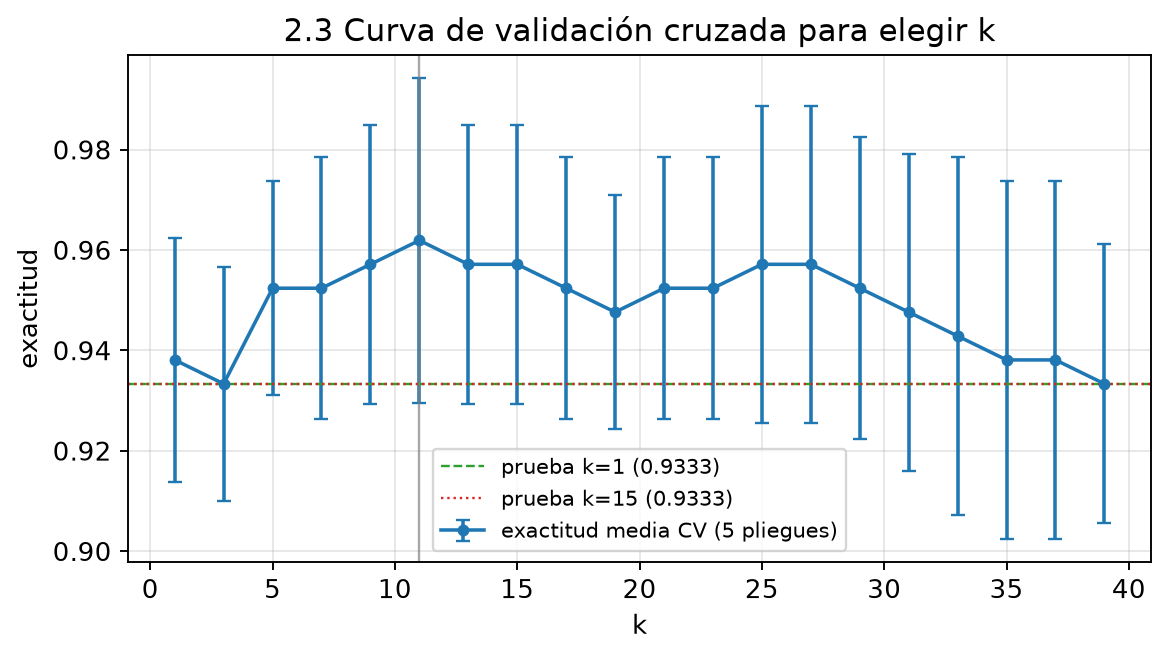
\includegraphics[width=0.78\textwidth]{fig_2_3_cv.png}
\caption{2.3 Curva de validación cruzada (5 pliegues) sobre el entrenamiento para
elegir $k$; las líneas horizontales marcan la exactitud de prueba de $k=1$ y
$k=15$ como referencia, no como criterio de selección.}
\label{fig:cv}
\end{figure}

%==========================================================================
\section{Punto 3: evaluación de un clasificador binario}

Etiquetas reales y predichas, con la clase $1$ como positiva:
\begin{equation}
y = [0,0,0,0,1,1,1,1,1,1], \qquad
\yhat = [0,1,0,0,1,0,1,1,0,1].
\end{equation}

\subsection{Matriz de confusión}

Filas: clase real; columnas: clase predicha. Recorriendo las diez posiciones:

\begin{table}[H]
\centering
\caption{3.1 Clasificación de cada observación.}
\label{tab:obs}
\begin{tabular}{cccccccccc}
\toprule
\# & 1 & 2 & 3 & 4 & 5 & 6 & 7 & 8 & 9/10 \\
\midrule
$y$ & 0 & 0 & 0 & 0 & 1 & 1 & 1 & 1 & 1, 1 \\
$\yhat$ & 0 & 1 & 0 & 0 & 1 & 0 & 1 & 1 & 0, 1 \\
Resultado & $TN$ & $FP$ & $TN$ & $TN$ & $TP$ & $FN$ & $TP$ & $TP$ & $FN$, $TP$ \\
\bottomrule
\end{tabular}
\end{table}

\begin{equation}
\text{Matriz de confusión} =
\begin{array}{c|cc}
 & \yhat = 0 & \yhat = 1 \\ \hline
y = 0 & TN = 3 & FP = 1 \\
y = 1 & FN = 2 & TP = 4
\end{array}
\qquad\Longrightarrow\qquad
\begin{aligned}
TP &= 4,\;& TN &= 3,\\
FP &= 1,\;& FN &= 2 .
\end{aligned}
\end{equation}

Comprobación: $TP+TN+FP+FN = 10$ observaciones; positivos reales
$TP+FN = 6$; negativos reales $TN+FP = 4$.

\subsection{Métricas}

\begin{align}
\text{Accuracy} &= \frac{TP+TN}{TP+TN+FP+FN} = \frac{4+3}{10} = 0.70\;\text{(70\,\%)},\\[2pt]
\text{Precision} &= \frac{TP}{TP+FP} = \frac{4}{4+1} = 0.80\;\text{(80\,\%)},\\[2pt]
\text{Recall} &= \frac{TP}{TP+FN} = \frac{4}{4+2} = \frac{2}{3} \approx 0.6667\;\text{(66.67\,\%)},\\[2pt]
F_1 &= \frac{2\,\text{Precision}\,\text{Recall}}{\text{Precision}+\text{Recall}}
= \frac{2\cdot 0.8\cdot \tfrac{2}{3}}{0.8+\tfrac{2}{3}}
= \frac{16/15}{22/15} = \frac{8}{11} \approx 0.7273\;\text{(72.73\,\%)}.
\end{align}

\paragraph{Qué evalúa cada medida.}
\begin{itemize}
\item \textbf{Accuracy}: proporción de aciertos sobre el total, contando
  positivos y negativos. Medida global y simétrica; sólo es informativa si las
  clases están balanceadas y ambos errores cuestan lo mismo.
\item \textbf{Precision} (valor predictivo positivo): de todo lo que el modelo
  marcó como positivo, qué fracción lo era realmente. Cuantifica el costo de las
  \emph{falsas alarmas} ($FP$); importa cuando un positivo predicho dispara una
  acción costosa (bloquear una cuenta, notificar a un cliente, iniciar un
  tratamiento invasivo).
\item \textbf{Recall} (sensibilidad o exhaustividad): de todos los positivos
  reales, qué fracción se detectó. Cuantifica el costo de los \emph{falsos
  negativos} ($FN$); importa cuando dejar pasar un positivo es grave (enfermedad,
  fraude, falla de un equipo).
\item $\boldsymbol{F_1}$: media armónica de precision y recall. Castiga el
  desequilibrio entre ambas: un modelo con precision $1.0$ y recall $0.1$ tiene
  $F_1 \approx 0.18$ aunque su «mitad» de desempeño sea perfecta. Útil con
  desbalance de clases cuando ambos tipos de error importan.
\end{itemize}

\subsection{Verificación en Python y análisis}

La verificación con \texttt{scikit-learn} reproduce exactamente los valores
manuales (Tabla~\ref{tab:verif}); el cuaderno incluye además aserciones
(\texttt{assert}) que fallan si el cálculo manual y el de la biblioteca difieren.

\begin{table}[H]
\centering
\caption{3.3 Cálculo manual frente a \texttt{scikit-learn}.}
\label{tab:verif}
\begin{tabular}{lcc}
\toprule
Medida & Manual & \texttt{scikit-learn} \\
\midrule
\texttt{confusion\_matrix} & $[3,\,1;\ 2,\,4]$ & $[3,\,1;\ 2,\,4]$\\
\texttt{accuracy\_score}  & $0.7000$ & $0.7000$\\
\texttt{precision\_score} & $0.8000$ & $0.8000$\\
\texttt{recall\_score}    & $0.6667$ & $0.6667$\\
\texttt{f1\_score}        & $0.7273$ & $0.7273$\\
\bottomrule
\end{tabular}
\end{table}

\begin{figure}[H]
\centering
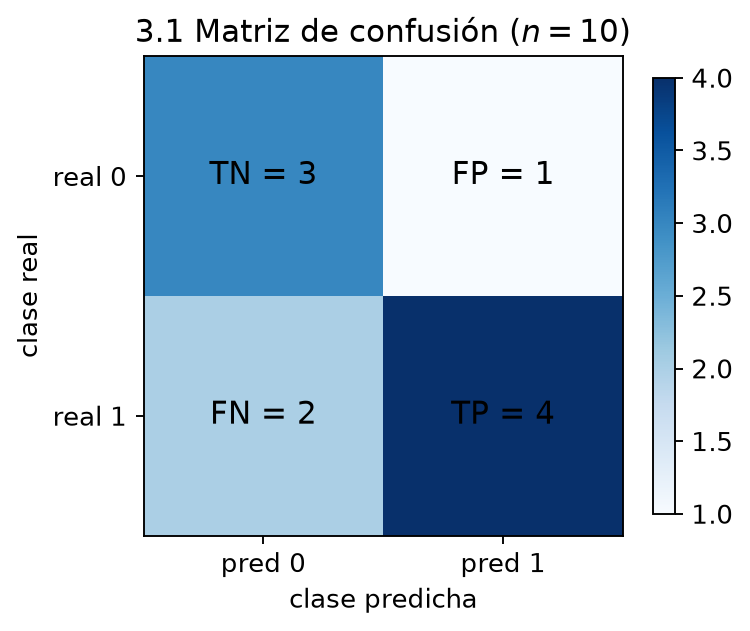
\includegraphics[width=0.45\textwidth]{fig_3_1_matriz.png}
\caption{3.1 Matriz de confusión del ejemplo (filas: clase real; columnas: clase
predicha).}
\label{fig:matriz}
\end{figure}

\paragraph{Dos situaciones en las que la exactitud por sí sola engaña.}

\begin{enumerate}
\item \textbf{Clases desbalanceadas.} Si el 95\,\% de los casos son negativos,
  un clasificador trivial que siempre responde «negativo» obtiene
  accuracy $= 0.95$ con recall $= 0$ para la clase positiva: nunca detecta un
  solo positivo. La exactitud es altísima y el modelo es inútil para el objetivo.
  En el cuaderno se ilustra con \texttt{DummyClassifier(strategy="most\_frequent")}
  sobre $95$ negativos y $5$ positivos: accuracy $0.95$, precision $0$, recall $0$
  y $F_1 = 0$.
\item \textbf{Costos asimétricos de los errores.} Un $FP$ y un $FN$ rara vez
  cuestan lo mismo. En tamizaje médico o detección de fraude, un $FN$ puede ser un
  daño grave mientras que un $FP$ sólo implica una verificación adicional; dos
  modelos con exactitud idéntica pueden diferir radicalmente en recall y
  precision, y la exactitud no distingue cuál de los dos errores se está
  cometiendo. El ejemplo del punto 3 lo muestra: accuracy $0.70$ oculta que se
  dejan pasar $2$ de $6$ positivos (recall 66.67\,\%) y que $1$ de cada $5$
  positivos predichos es falso ($FP$).
\end{enumerate}

\noindent
Otras dos situaciones, por completitud: conjuntos muy pequeños, donde una sola
observación mueve varios puntos porcentuales de exactitud, y problemas
multiclase, donde la exactitud global promedia clases con desempeños muy
distintos y hace falta la matriz de confusión (o métricas por clase) para verlo.

%==========================================================================
\section{Conclusiones}

\begin{enumerate}
\item \textbf{Frontera lineal.} La regla $\yhat = \operatorname{sign}(\w^\top\x+b)$
  usa el signo del puntaje, y $\w$ es normal a la recta de decisión. Con
  $\w = (1,2)^\top$, $b=-3$ la frontera $x_2 = 1.5 - 0.5x_1$ asigna $-1$ a
  $x_1=(0,0)$ y $x_2=(1,0)$, y $+1$ a $x_3=(2,1)$ y $x_4=(3,1)$.
\item \textbf{Perceptrón.} La actualización sobre una observación mal clasificada
  incrementa su margen funcional en $\eta(\lVert \x_i\rVert_2^2+1) > 0$, con
  independencia del error previo; el margen geométrico no es necesariamente
  monótono porque $\lVert\w\rVert$ también cambia. En el ejercicio numérico
  ($\w=0$, $b=0$, $\eta=0.5$, $\x=(2,1)$, $y=+1$) sí hay error, y resultan
  $\w_{\text{nuevo}} = (1,0.5)^\top$, $b_{\text{nuevo}} = 0.5$ y
  $m_{\text{nuevo}} = 3$, consistente con la fórmula de 1.2.
\item \textbf{k-NN.} El orden de cercanía a $q=(1,1)$ es
  $x_5 \prec x_2 \prec x_1 \prec x_3 \prec x_4$ y la predicción pasa de \textbf{B}
  ($k=1$) a \textbf{A} ($k=3$) y de nuevo a \textbf{B} ($k=5$): $k$ controla el
  compromiso sesgo--varianza. Sobre \texttt{make\_moons}
  ($N=300$, \texttt{noise=0.20}) las exactitudes de prueba son $0.9333$
  ($k=1$), $0.9556$ ($k=5$) y $0.9333$ ($k=15$); $k=1$ memoriza el entrenamiento
  (accuracy $1.0000$) con frontera irregular y $k=5$ generaliza mejor. La
  selección formal de $k$ se hace por validación cruzada de 5 pliegues sobre el
  entrenamiento, que aquí escoge $k=11$ (CV $0.9619$, prueba $0.9667$), nunca
  mirando el conjunto de prueba.
\item \textbf{Evaluación.} Para el ejemplo del punto 3,
  $TP=4$, $TN=3$, $FP=1$, $FN=2$; accuracy $0.70$, precision $0.80$, recall
  $0.6667$ y $F_1 = 8/11 \approx 0.7273$, verificados con \texttt{scikit-learn}.
  La exactitud sola engaña con clases desbalanceadas o con costos asimétricos de
  los errores; precision, recall, $F_1$ y la matriz de confusión son
  imprescindibles para interpretar el desempeño.
\end{enumerate}

%==========================================================================
\section*{Reproducibilidad}
\addcontentsline{toc}{section}{Reproducibilidad}

El cuaderno \texttt{solucion\_taller.ipynb} es autocontenido: no lee archivos
externos, genera sus propios datos y sólo requiere \texttt{numpy},
\texttt{scikit-learn} y \texttt{matplotlib}.

\paragraph{Google Colab (recomendado).} Subir el archivo a Drive (o
\emph{Archivo $\to$ Subir cuaderno}) y ejecutar
\emph{Entorno de ejecución $\to$ Ejecutar todo}. Colab ya trae las tres
bibliotecas; la primera celda de código las comprueba y, si faltara alguna, la
instala con \texttt{pip}. Las figuras se escriben en \texttt{figuras/} y el
resumen numérico en \texttt{resultados.json} dentro del directorio de trabajo de
la sesión (\texttt{/content} en Colab), sin afectar la reproducibilidad de los
resultados.

\paragraph{Local.} Python 3.10 o superior con las tres bibliotecas:

\begin{lstlisting}[language=bash,numbers=none]
python3 -m venv .venv
.venv/bin/python -m pip install numpy scikit-learn matplotlib jupyter
.venv/bin/jupyter notebook solucion_taller.ipynb   # Ejecutar todo
\end{lstlisting}

\noindent
El cuaderno fija \texttt{np.random.seed(42)} y usa \texttt{random\_state=42} en
\texttt{make\_moons}, \texttt{train\_test\_split} y \texttt{StratifiedKFold}; dos
ejecuciones completas producen exactamente los mismos resultados. Versiones de
desarrollo: Python 3.14, \texttt{numpy 2.5.4}, \texttt{scikit-learn 1.9.1},
\texttt{matplotlib 3.11.2} (el cuaderno imprime las versiones efectivas al
iniciar).

\appendix
\section{Código de las partes implementadas manualmente}

\paragraph{Perceptrón: predicción y actualización (1.3).}
\begin{lstlisting}
def predecir(w, b, x):
    return 1 if w @ x + b > 0 else -1

def actualizar(w, b, x, y, eta):
    return w + eta * y * x, b + eta * y

w, b, eta, x, y = np.zeros(2), 0.0, 0.5, np.array([2.0, 1.0]), 1.0
if y * (w @ x + b) <= 0:                    # hay error -> se actualiza
    w, b = actualizar(w, b, x, y, eta)
    print(w, b, y * (w @ x + b))            # [1.  0.5] 0.5 3.0
\end{lstlisting}

\paragraph{k-NN con votación mayoritaria manual (2.1).}
\begin{lstlisting}
def knn_manual(q, X, clases, k):
    d = np.linalg.norm(X - q, axis=1)       # distancia euclidiana
    idx = np.argsort(d, kind="stable")[:k]  # k vecinos mas cercanos
    votos = {}
    for c in clases[idx]:
        votos[str(c)] = votos.get(str(c), 0) + 1
    return sorted(votos.items(), key=lambda kv: (-kv[1], kv[0]))[0][0]
\end{lstlisting}

\paragraph{Protocolo experimental de 2.2.}
\begin{lstlisting}
X, y = make_moons(n_samples=300, noise=0.20, random_state=42)
X_tr, X_te, y_tr, y_te = train_test_split(
    X, y, test_size=0.30, stratify=y, random_state=42)
for k in (1, 5, 15):
    m = KNeighborsClassifier(n_neighbors=k).fit(X_tr, y_tr)
    print(k, accuracy_score(y_tr, m.predict(X_tr)),
             accuracy_score(y_te, m.predict(X_te)))

cv = StratifiedKFold(n_splits=5, shuffle=True, random_state=42)
for k in range(1, 41, 2):
    print(k, cross_val_score(KNeighborsClassifier(n_neighbors=k),
                             X_tr, y_tr, cv=cv).mean())
\end{lstlisting}

\paragraph{Métricas: cálculo manual y verificación (3).}
\begin{lstlisting}
TP = int(np.sum((y == 1) & (yhat == 1)))
TN = int(np.sum((y == 0) & (yhat == 0)))
FP = int(np.sum((y == 0) & (yhat == 1)))
FN = int(np.sum((y == 1) & (yhat == 0)))

acc = (TP + TN) / (TP + TN + FP + FN)          # 0.70
prec = TP / (TP + FP)                          # 0.80
rec = TP / (TP + FN)                           # 0.6667
f1 = 2 * prec * rec / (prec + rec)             # 0.7273

assert np.array_equal(np.array([[TN, FP], [FN, TP]]),
                      confusion_matrix(y, yhat, labels=[0, 1]))
\end{lstlisting}

\end{document}
